\chapter{Masked language models}



\section{Bidirectional transformer encoder}

\begin{description}
    \item[Transformer encoder] \marginnote{Transformer encoder}
        Architecture that produces contextual embeddings by considering both left-to-right and right-to-left context.

        \begin{remark}
            This architecture does feature extraction and is more suited for classification tasks.
        \end{remark}

        \begin{description}
            \item[Architecture]
                Similar to a transformer decoder, but self-attention is not causal.

                \begin{figure}[H]
                    \centering
                    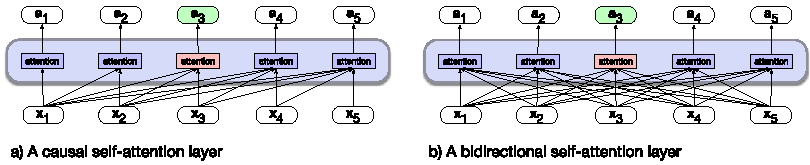
\includegraphics[width=0.75\linewidth]{./img/_decoder_vs_encoder.pdf}
                \end{figure}
        \end{description}
\end{description}


\subsection{Masked language modelling}

\begin{description}
    \item[Masked language modelling] \marginnote{Masked language modelling}
        Main training task of transformer encoders. It consists of predicting missing or corrupted tokens in a sequence.

        \begin{remark}
            Transformer encoders output embeddings. For training purposes, a head to output a distribution over the vocabulary is added.
        \end{remark}

        \begin{example}
            Given a training corpus, BERT is trained by randomly sampling $15\%$ of the tokens in the training data and either:
            \begin{itemize}
                \item Mask it with a special \texttt{[MASK]} token ($80\%$ of the time).
                \item Replace it with a different token ($10\%$ of the time).
                \item Do nothing ($10\%$ of the time).
            \end{itemize}

            \begin{figure}[H]
                \centering
                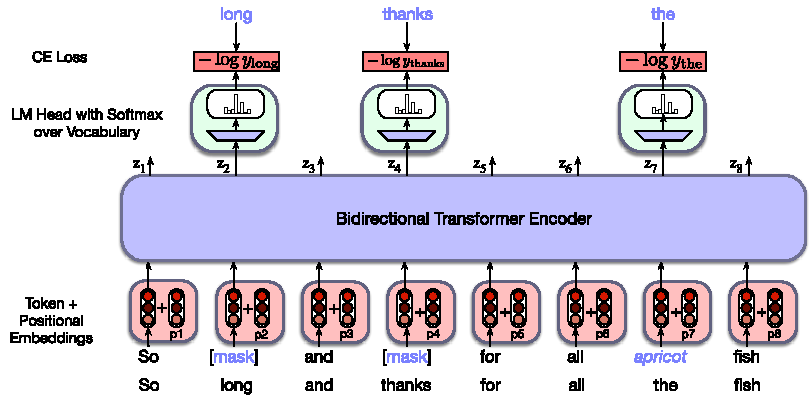
\includegraphics[width=0.6\linewidth]{./img/_bert_training.pdf}
            \end{figure}

            \indenttbox
            \begin{remark}
                BERT's training approach is inefficient as masks are determined before training and only $15\%$ of the corpus tokens are actually used for training. Other models (e.g., RoBERTa), dynamically determine the mask at training time, allowing for more variety.
            \end{remark}
        \end{example}
\end{description}